\chapter{Contribution \& system design}

This chapter presents the central contribution of this work. First we start by presenting our objectives and move into introducing our creation, with diagrams, figures and descriptions.

\section{Work objectives}

The goal of this work is to propose a decentralized electronic voting system. The central piece to creating this system is its design and architecture, so after reviewing and analyzing similar proposed works \cite{khouryDecentralizedVotingPlatform2018}\cite{angsuchotmeteeBlockVOTEArchitectureBlockchainbased2019}\cite{ahlkvistDecentralizedVotingSystem2019} and traditional voting practices, we created our own design that remedies some of what we perceived to be shortcomings in previous works.

\section{Literature \& related works review}

We present in this section solutions that attempt to integrate Blockchain into electronic voting to enable decentralization of voting services. We then present the main differences between these works and our design and highlight the added value.

\textit{a) Decentralized Voting Platform Based on Ethereum
Blockchain:} David Khoury et al. discuss in their paper entitled "Decentralized Voting Platform Based on Ethereum
Blockchain"\cite{khouryDecentralizedVotingPlatform2018} a decentralized voting solution based on Ethereum Blockchain. It states that their solution solves the trust issues by relying on Blockchain technology. Users in this system are authenticated through their mobile phone number and their phones are used to cast their votes. Here is where our approach starts to differ, allowing voters to vote from their own devices exposes the voter to the potential danger of having their authenticated personal devices taken over by malicious parties and votes being cast in their name without their consent. Also, their system architecture relies on a management server that sits below the administrator web interface and carries the interactions with the Blockchain, which makes the system susceptible to \gls{DDoS}s.

\textit{b) BlockVOTE: An Architecture of a Blockchain-based Electronic Voting System:} in this paper entitled "BlockVOTE: An Architecture of a Blockchain-based Electronic Voting System"\cite{angsuchotmeteeBlockVOTEArchitectureBlockchainbased2019}, Chinnapong Angsuchotmetee and Pisal Setthawong propose a decentralized Blockchain-based electronic voting system and then give an analysis of both technical and management aspects on the possibility of adopting the proposed system. BlockVOTE system does not include the entity responsible for authenticating authorized voters, although, in the paper, the authors state that authentication is performed before any vote is cast. Also unlike our system, they propose that a new smart contract is deployed for every new event, while for our design we judge that to be unnecessary and prefer to reuse the same deployed once smart contract.
 
\textit{c) A Decentralized Voting System:} Jack Ahlkvist
et al. from Chalmers University of Technology investigate in their paper "A Decentralized Voting System"\cite{ahlkvistDecentralizedVotingSystem2019} the possibility of a decentralized voting system and explore the possible challenges regarding privacy, correctness and integrity. Using the Ethereum blockchain and various smart contracts. Their proposed solution stores authorized voters' ID on the Blockchain, which in the case of a national election would mean millions of issued IDs. Storing data on the Blockchain is always more secure and reliable, however, it is also very costly.

\section{System design}

In this section, we introduce our proposed voting system that aims to solve some of the barriers that traditional voting systems have. Also remedy some of the shortcomings we perceived in similar proposed works.

\subsection{Architecture}

\begin{figure}[H]
	\centering
		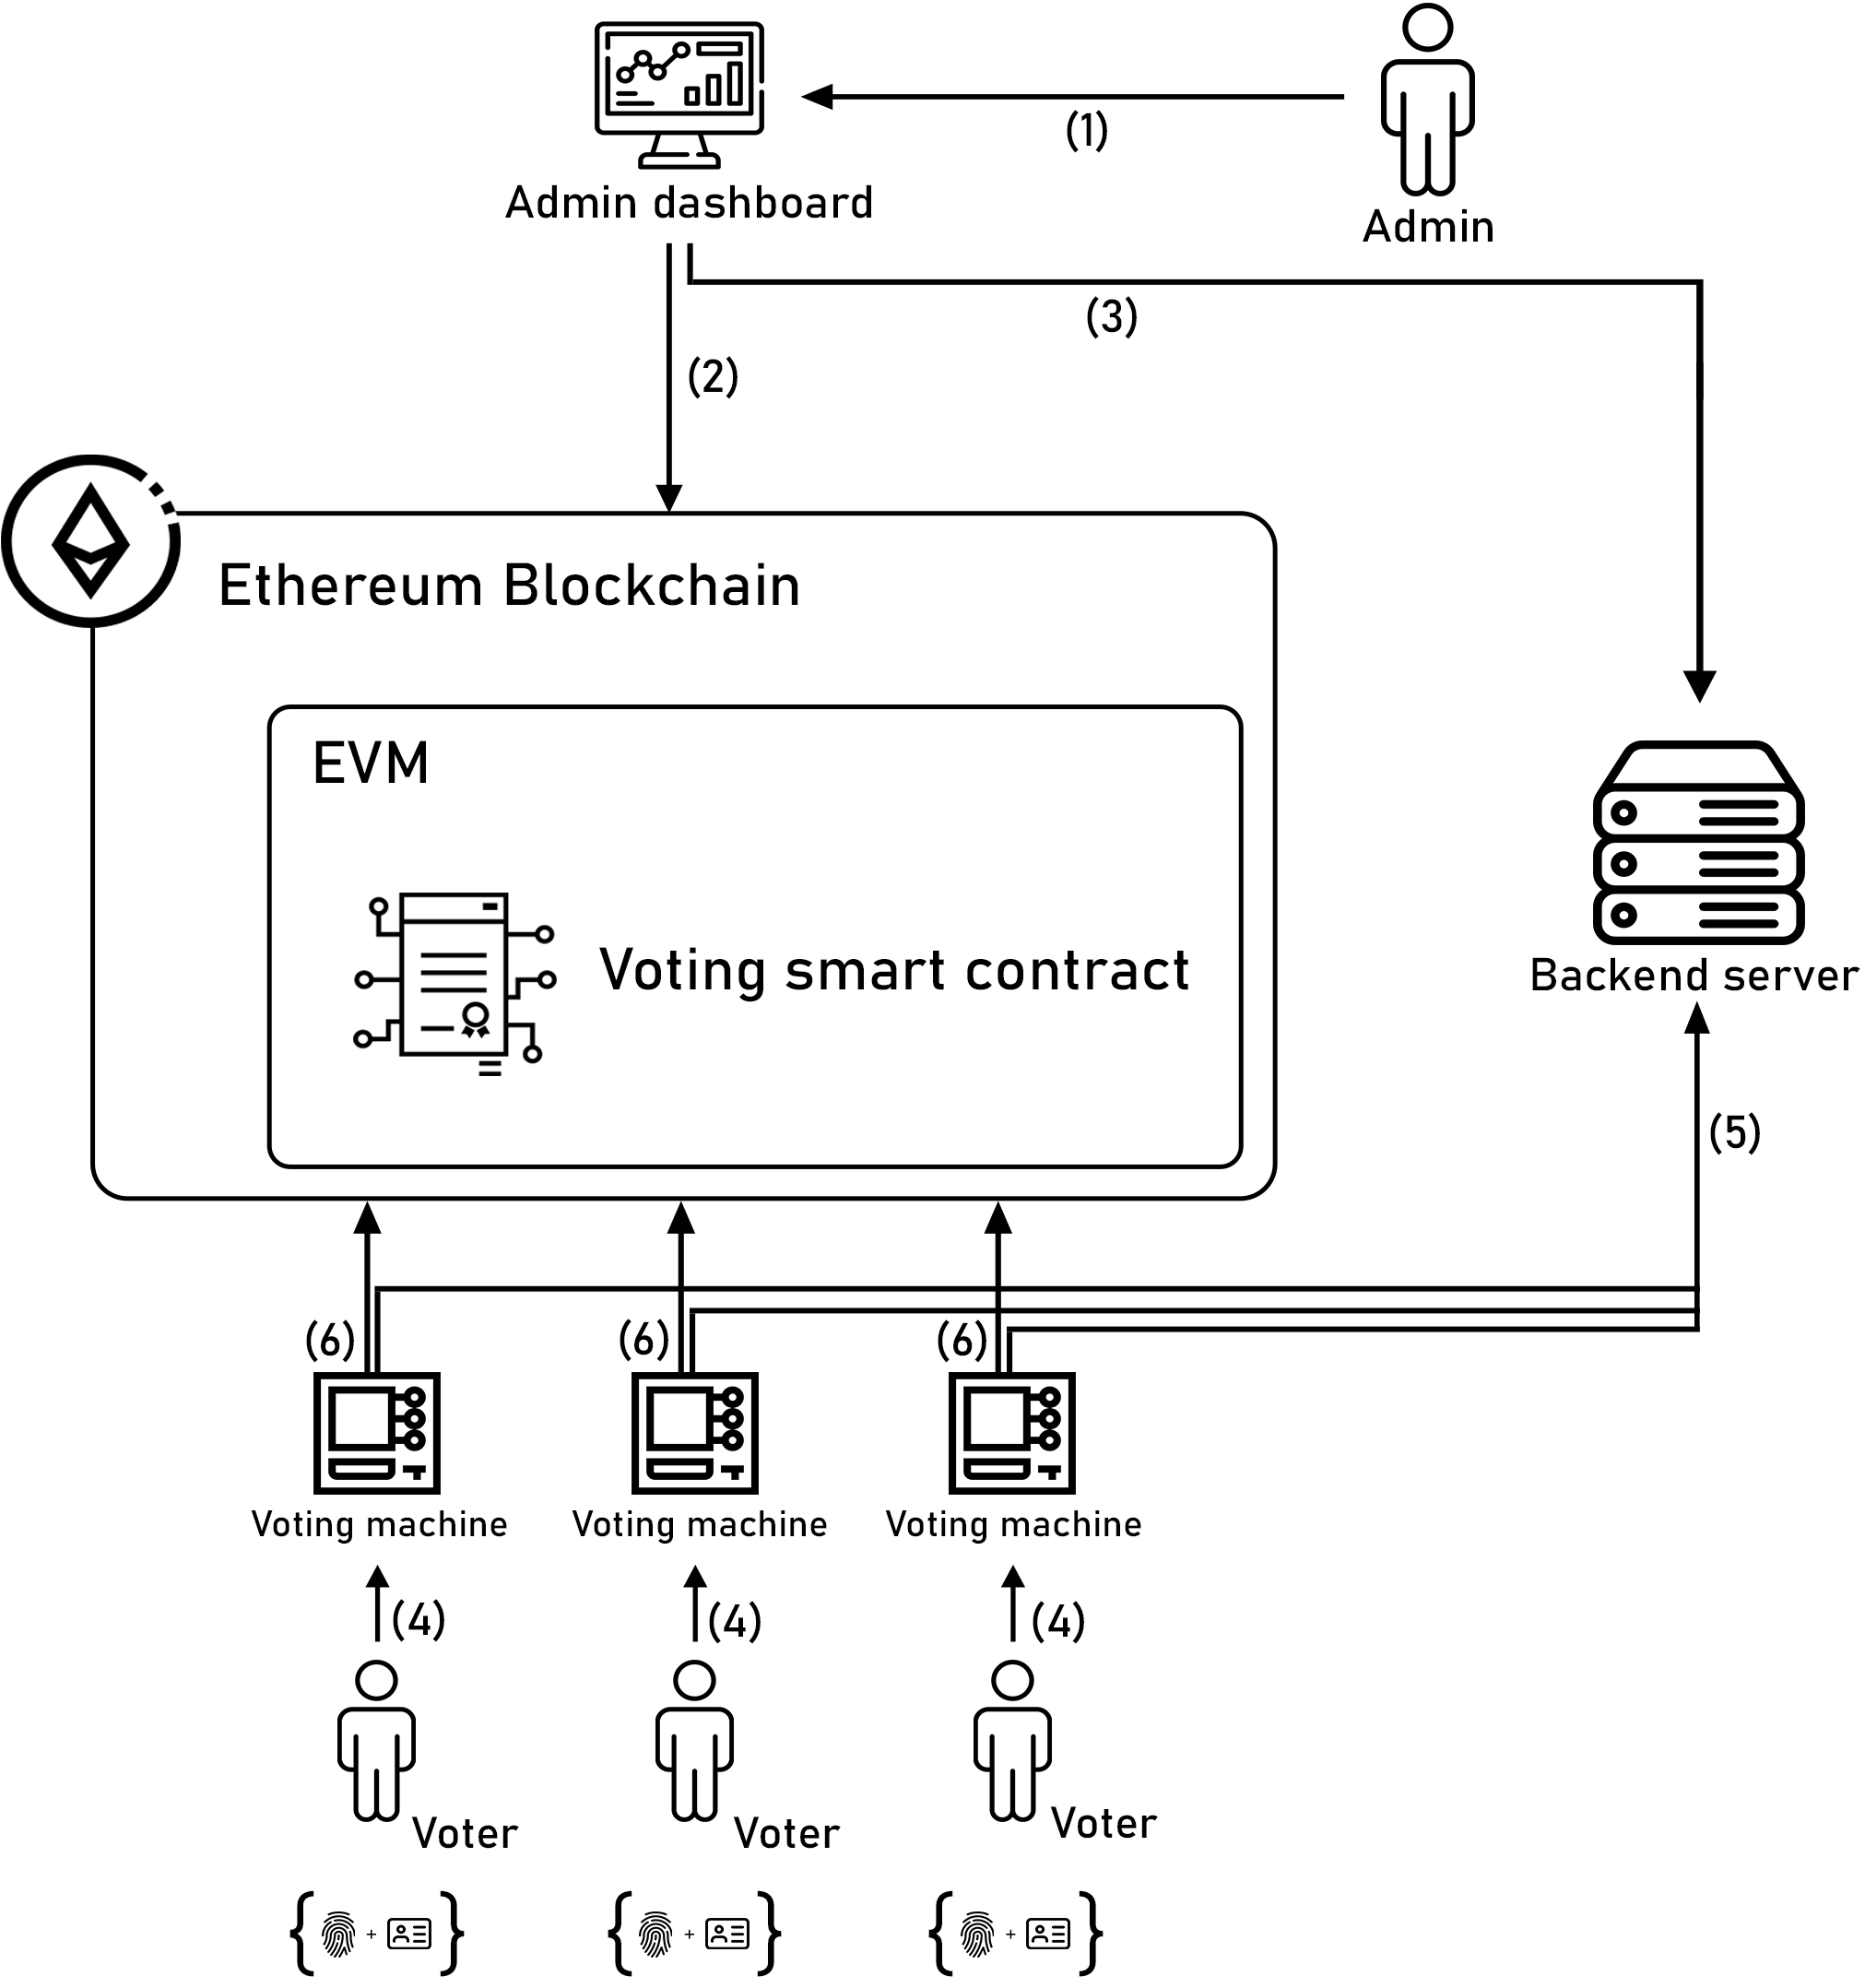
\includegraphics[width=12cm]{images/chapter3/architecture.png}
		\caption{{\footnotesize High level architecture of the proposed system and the interaction between its components}}
\end{figure}

\begin{list}{}{}
\item \textbf{(1)} The admin operating the dashboard launches and monitors voting events
\item \textbf{(2)} Essential data (candidates name and id, event title, start \& finish dates) are saved in the Blockchain along with the list of authorized accounts that can interact with the smart contract.
\item \textbf{(3)} Secondary data that is of less importance is saved to the regular (centralized) backend server.
\item \textbf{(4)} Voters authenticate themselves to the polling machines (using biometric means) and cast their vote for a candidate of their choosing
\item \textbf{(5)} Voting machines use the backend server to verify the identity of the voter and to fetch secondary data required for the displaying of candidates
\item \textbf{(6)} Voting machines saves the submitted choice to the Blockchain by launching a transaction that increments the vote count of the chosen candidate
\end{list}

\subsection{Diagrams}
\subsubsection{Admin sequence diagram}

\begin{figure}[H]
	\centering
		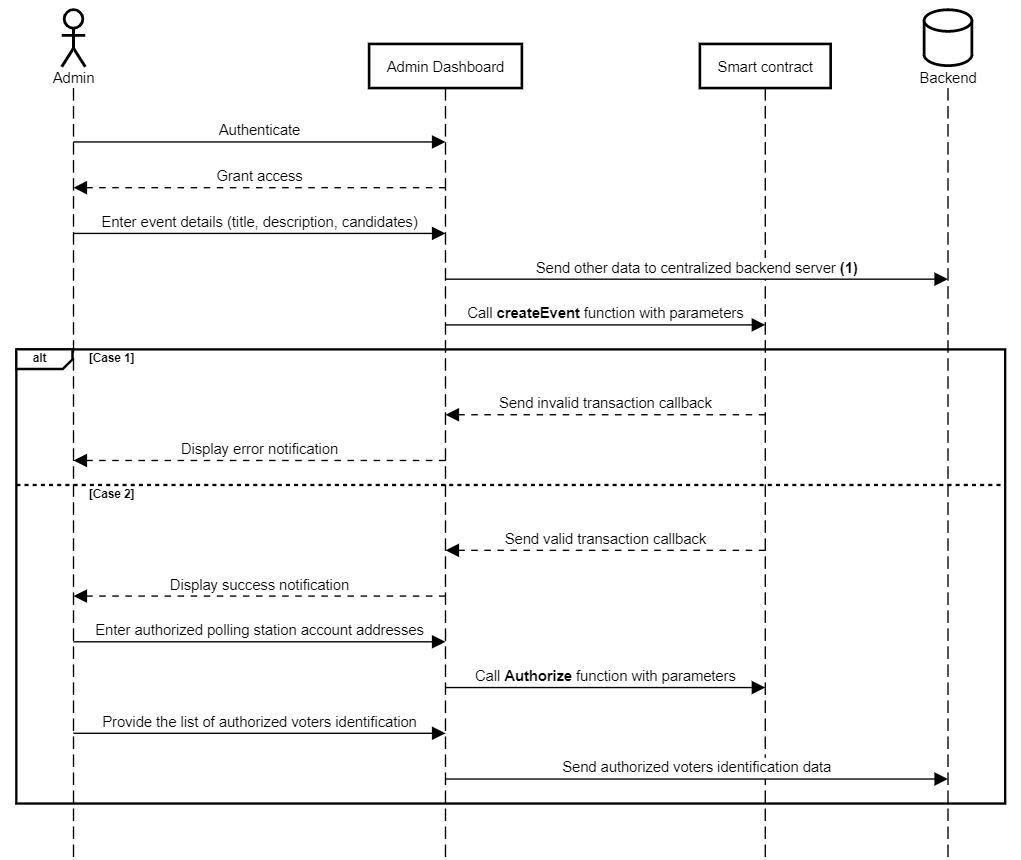
\includegraphics[width=14cm]{images/chapter3/admin_sequence_diagram.png}
		\caption{{\footnotesize Sequence diagram of the process of creating and launching a new voting event}}
\end{figure}

Launching an election requires that the administrator get access to the administration dashboard which has its access restricted by digital or physical boundaries or both, using the dashboard the administrator accesses the event creation form, in which he fills the information for the event. The information provided will be divided on the basis of their level of criticality, for example, candidates' pictures and lengthy descriptions are deemed to be less critical to the vote-counting so they're stored in a regular backend server. Also, information required for the authentication of voters is also stored on the regular backend servers.

Next, the administrator is tasked with providing the account addresses of the Ethereum accounts running on each voting machine, this list will be the list of the Ethereum account addresses allowed to interact with the smart contract and alter the vote count of any candidates by incrementing it.

\subsubsection{Voter sequence diagram}

\begin{figure}[H]
	\centering
		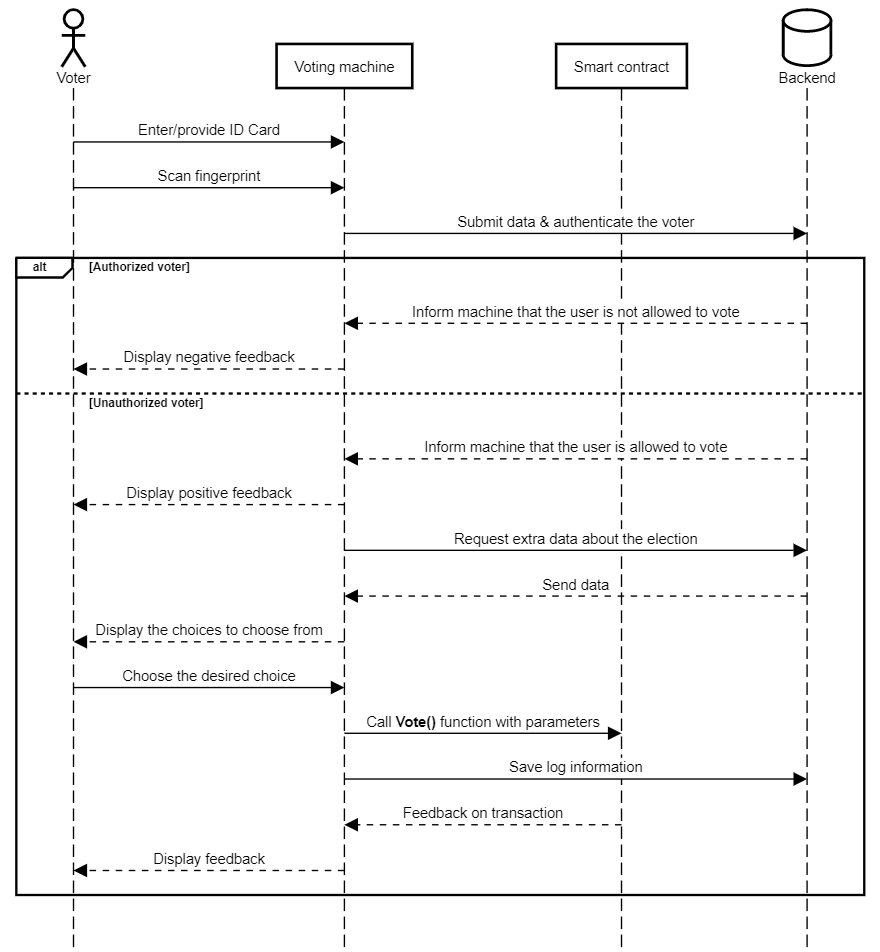
\includegraphics[width=14cm]{images/chapter3/voter_sequence_diagram.png}
		\caption{{\footnotesize Sequence diagram of the process of casting a vote}}
\end{figure}

The process of casting a vote is initiated when a voter first enters a polling station, then proceeds to a vacant voting machine, the machine should be equipped with an ID Card reader and fingerprint scanner to conduct a biometric identity check. the information obtained will be checked against the records saved on the backend server. In case the person is identified as an authorized voter; meeting whatever the requirements listed by the entity organizing the voting event (for example an entity can enforce one single vote per household or set the minimum age for participation to 50), a list of choices will be displayed to the voter to choose from in an intuitive manner after the voter makes his choice and submits it, the voting machine performance an Ethereum transaction to the smart contract by calling the appropriate function that will result in incrementing the vote count of that particular candidate, also log information about the vote will be saved to the backend server.
